\documentclass[11pt,a4paper]{article}
\usepackage[utf8]{inputenc}
\usepackage[T1]{fontenc}
\usepackage{amsmath,amssymb}
\usepackage{graphicx}
\usepackage{booktabs}
\usepackage{multirow}
\usepackage{hyperref}
\usepackage[margin=1in]{geometry}
\usepackage{natbib}
\usepackage{xcolor}
\usepackage{float}
\usepackage{caption}
\usepackage{subcaption}
\usepackage{setspace}
\usepackage{lineno}

\linenumbers
\onehalfspacing

\title{Population-Stratified Germline Indel Mutation Spectra Reveal Differential Mutagenic Process Contributions Across Diverse Human Populations}

\author{Computational Genomics Analysis}

\date{}

\begin{document}

\maketitle

\begin{center}
\fbox{%
\parbox{0.92\textwidth}{%
\centering\large\bfseries\color{red}
⚠ AI-GENERATED CONTENT — FOR SYSTEM EVALUATION ONLY ⚠\\[4pt]
\normalsize\mdseries\color{black}
This paper was produced entirely by an AI agent conducting autonomous experiments and writing.
It is part of a controlled study to evaluate AI research automation systems and is \textbf{not} peer-reviewed.
\textbf{Do not treat the scientific claims herein as validated research.}
Please exercise critical judgment when reading.
}%
}
\end{center}
\vspace{8pt}

\begin{abstract}
Small insertions and deletions (indels) represent the second most abundant class of genetic variation in human genomes, yet their mutation spectrum variation across populations remains poorly characterized compared to single nucleotide variants (SNVs). Here, we present a comprehensive analysis of 8,995,003 germline indels across 3,202 individuals from 26 populations spanning five continental super-populations, using the high-coverage (30$\times$) 1000 Genomes Project dataset. We classified indels into a 52-channel mutation spectrum based on type (insertion/deletion), size (1--50+ bp), and base composition, augmented with homopolymer context for single-nucleotide indels. Our analysis reveals highly significant population-specific patterns in the germline indel spectrum ($\chi^2 = 3{,}465.58$, $p < 10^{-300}$), with all 52 channels showing significant differentiation after Bonferroni correction. African populations exhibit a distinctive deletion-enriched spectrum (DEL/INS ratio = 1.155 vs. 1.039 in East Asians, $p < 10^{-200}$) with particularly elevated GC-context single-nucleotide deletions (1.27-fold enrichment relative to East Asian populations, 4.73\% vs. 3.72\%). Conversely, East Asian populations show enrichment for AT-context insertions in homopolymer runs, suggesting population-specific variation in replication slippage rates. Non-negative matrix factorization (NMF) decomposition identifies two principal germline indel signatures: an AT-dominated replication slippage signature enriched in East Asian and European populations, and a GC-enriched deletion signature with contributions from non-homopolymer mutagenic processes enriched in African populations. Jensen-Shannon divergence analysis confirms that African populations harbor the most divergent indel spectrum (JSD = 0.038 vs. East Asian), while European and South Asian populations show the greatest similarity (JSD = 0.003). These findings reveal previously uncharacterized population-level variation in germline indel mutagenesis and provide new insights into the differential contributions of mutagenic processes across human populations.
\end{abstract}

\textbf{Keywords:} germline indels, mutation spectrum, population genetics, 1000 Genomes Project, mutagenic processes, replication slippage, NMF signatures

\section{Introduction}

The characterization of human genetic variation is fundamental to understanding population history, disease susceptibility, and the mechanisms of mutagenesis. While single nucleotide variants (SNVs) have been the primary focus of population genetic studies, small insertions and deletions (indels) represent the second most abundant class of variation in human genomes \citep{1000genomes2015,byrska2022high}. Indels contribute substantially to human phenotypic diversity and disease risk, with approximately 1.5--2 million short indels segregating in any individual genome \citep{mullaney2010small,montgomery2013mutation}.

The mutational processes that generate indels differ fundamentally from those producing SNVs. While SNVs arise predominantly through base misincorporation during DNA replication and chemical modification of bases, indels are generated through mechanistically distinct processes including replication slippage at microsatellites and homopolymer tracts, template switching during DNA repair, errors in non-homologous end joining, and microhomology-mediated recombination \citep{levinson1987slipped,pearson2005repeat,chuzhanova2003meta}. Each of these mechanisms produces indels with characteristic size distributions and sequence contexts, analogous to how distinct mutational processes produce recognizable SNV signatures in cancer genomes \citep{alexandrov2013signatures,alexandrov2020repertoire}.

In the cancer genomics field, the analysis of mutational signatures has been transformative. The Catalogue of Somatic Mutations in Cancer (COSMIC) has catalogued 18 indel signatures (ID1--ID18) associated with specific mutagenic processes such as defective DNA mismatch repair, polymerase slippage, and tobacco exposure \citep{alexandrov2020repertoire}. However, the systematic characterization of germline indel mutation spectra---and particularly their variation across human populations---has received far less attention.

Previous studies of population-level indel variation have focused primarily on overall burden and frequency spectra \citep{1000genomes2015,mills2011natural}, with limited examination of the compositional spectrum of indel mutations across populations. The recent release of high-coverage (30$\times$) whole genome sequencing data from the 1000 Genomes Project for 3,202 individuals from 26 globally diverse populations \citep{byrska2022high} provides an unprecedented opportunity to characterize germline indel spectra at fine resolution across human populations. The substantially improved indel calling sensitivity and specificity of high-coverage sequencing compared to the original low-coverage (4--8$\times$) data \citep{byrska2022high} is particularly important, as indel detection is more sensitive to sequencing depth than SNV detection.

Here, we present a comprehensive population-stratified analysis of the germline indel mutation spectrum using the 1000 Genomes high-coverage dataset. We define a 52-channel indel classification system incorporating type (insertion vs. deletion), size, base composition, and homopolymer context, and apply it to nearly 9 million indels across 22 autosomes. Our analysis reveals highly significant population-specific patterns in the indel spectrum, with African populations showing a distinctively deletion-enriched spectrum and elevated GC-context mutations, while East Asian populations exhibit enrichment for AT-context insertions in homopolymer runs. Using non-negative matrix factorization (NMF), we decompose the germline indel spectrum into component signatures and demonstrate their differential contributions across populations. These findings provide new insights into the population-level variation of mutagenic processes shaping human indel diversity.

\section{Materials and Methods}

\subsection{Dataset}

We analyzed the high-coverage (30$\times$) 1000 Genomes Project dataset \citep{byrska2022high}, which comprises 3,202 individuals from 26 populations across five continental super-populations: African (AFR, $n = 893$), American (AMR, $n = 490$), East Asian (EAS, $n = 585$), European (EUR, $n = 633$), and South Asian (SAS, $n = 601$). We used the phased SNV/INDEL/SV call set (release 20220422) aligned to the GRCh38 reference genome. Variant calls were obtained from the publicly available resource at the International Genome Sample Resource.

\subsection{Indel Extraction and Filtering}

Indels were extracted from the phased VCF files for all 22 autosomes using bcftools (v1.20) \citep{danecek2021twelve}. We retained all biallelic indels passing quality filters included in the original call set. For each indel, we recorded the chromosome, position, reference allele, alternate allele, allele count (AC), allele number (AN), and allele frequency (AF). Multi-allelic sites were treated as separate entries. A total of 8,995,003 autosomal indels were retained for analysis.

\subsection{Indel Classification System}

Each indel was classified along three dimensions:

\begin{enumerate}
\item \textbf{Type}: Insertion (INS) or deletion (DEL), determined by comparing the lengths of reference and alternate alleles.
\item \textbf{Size}: The absolute difference in length between reference and alternate alleles, binned into nine categories: 1 bp, 2 bp, 3 bp, 4 bp, 5 bp, 6--10 bp, 11--20 bp, 21--50 bp, and $>$50 bp.
\item \textbf{Base composition}: For 1 bp indels, classified as AT (A or T) or GC (C or G). For multi-base indels, classified as AT-rich ($>$70\% A/T), GC-rich ($>$70\% G/C), or mixed.
\end{enumerate}

The combination of these three dimensions yielded 52 distinct channels. Additionally, for 1 bp indels, we determined the homopolymer run length at each position by querying the GRCh38 reference genome sequence flanking each variant position using pysam (v0.22.1) \citep{pysam}. The homopolymer length was defined as the total number of consecutive identical bases spanning the indel position.

\subsection{Per-Population Allele Frequency Computation}

To compute super-population-specific allele frequencies, we extracted indel genotypes for each super-population independently using bcftools with population-specific sample lists. For each variant, population-specific allele counts (AC) and allele numbers (AN) were computed. A variant was considered segregating in a population if its population-specific AC $> 0$.

\subsection{Statistical Analysis}

\subsubsection{Spectrum Comparison}

Population differences in indel spectra were assessed using the chi-square test of independence on the raw count matrix (populations $\times$ channels). Effect size was quantified using Cram\'er's V statistic. Channel-specific differentiation was evaluated using per-channel chi-square tests with Bonferroni correction for multiple testing.

\subsubsection{Population Divergence Measures}

Pairwise population divergence was quantified using: (i) cosine similarity between normalized spectrum vectors, (ii) Jensen-Shannon divergence (JSD), and (iii) hierarchical clustering using average linkage with cosine distance.

\subsubsection{Deletion-to-Insertion Ratio}

The deletion-to-insertion (DEL/INS) ratio was computed for each super-population as the total number of segregating deletions divided by insertions. Deviation from the null expectation of equal deletion and insertion rates was tested using the binomial test.

\subsubsection{NMF Signature Decomposition}

Non-negative matrix factorization (NMF) \citep{lee1999learning} was applied to the population $\times$ channel count matrix to decompose the indel spectrum into component signatures. We tested ranks $k = 2, 3, 4$ and evaluated model fit using reconstruction error. NMF was implemented using scikit-learn (v1.7.2) \citep{pedregosa2011scikit} with random initialization and 1,000 maximum iterations.

\subsection{Software and Reproducibility}

All analyses were performed using Python 3.12 with pandas (v2.2.3), NumPy (v2.2.6), SciPy (v1.13.1), scikit-learn (v1.7.2), matplotlib (v3.10.1), and seaborn (v0.13.2). Variant processing used bcftools (v1.20) and plink2. Reference genome queries used pysam (v0.22.1) with the GRCh38 assembly.

\section{Results}

\subsection{Genome-Wide Germline Indel Landscape}

\begin{figure}[!ht]
\centering
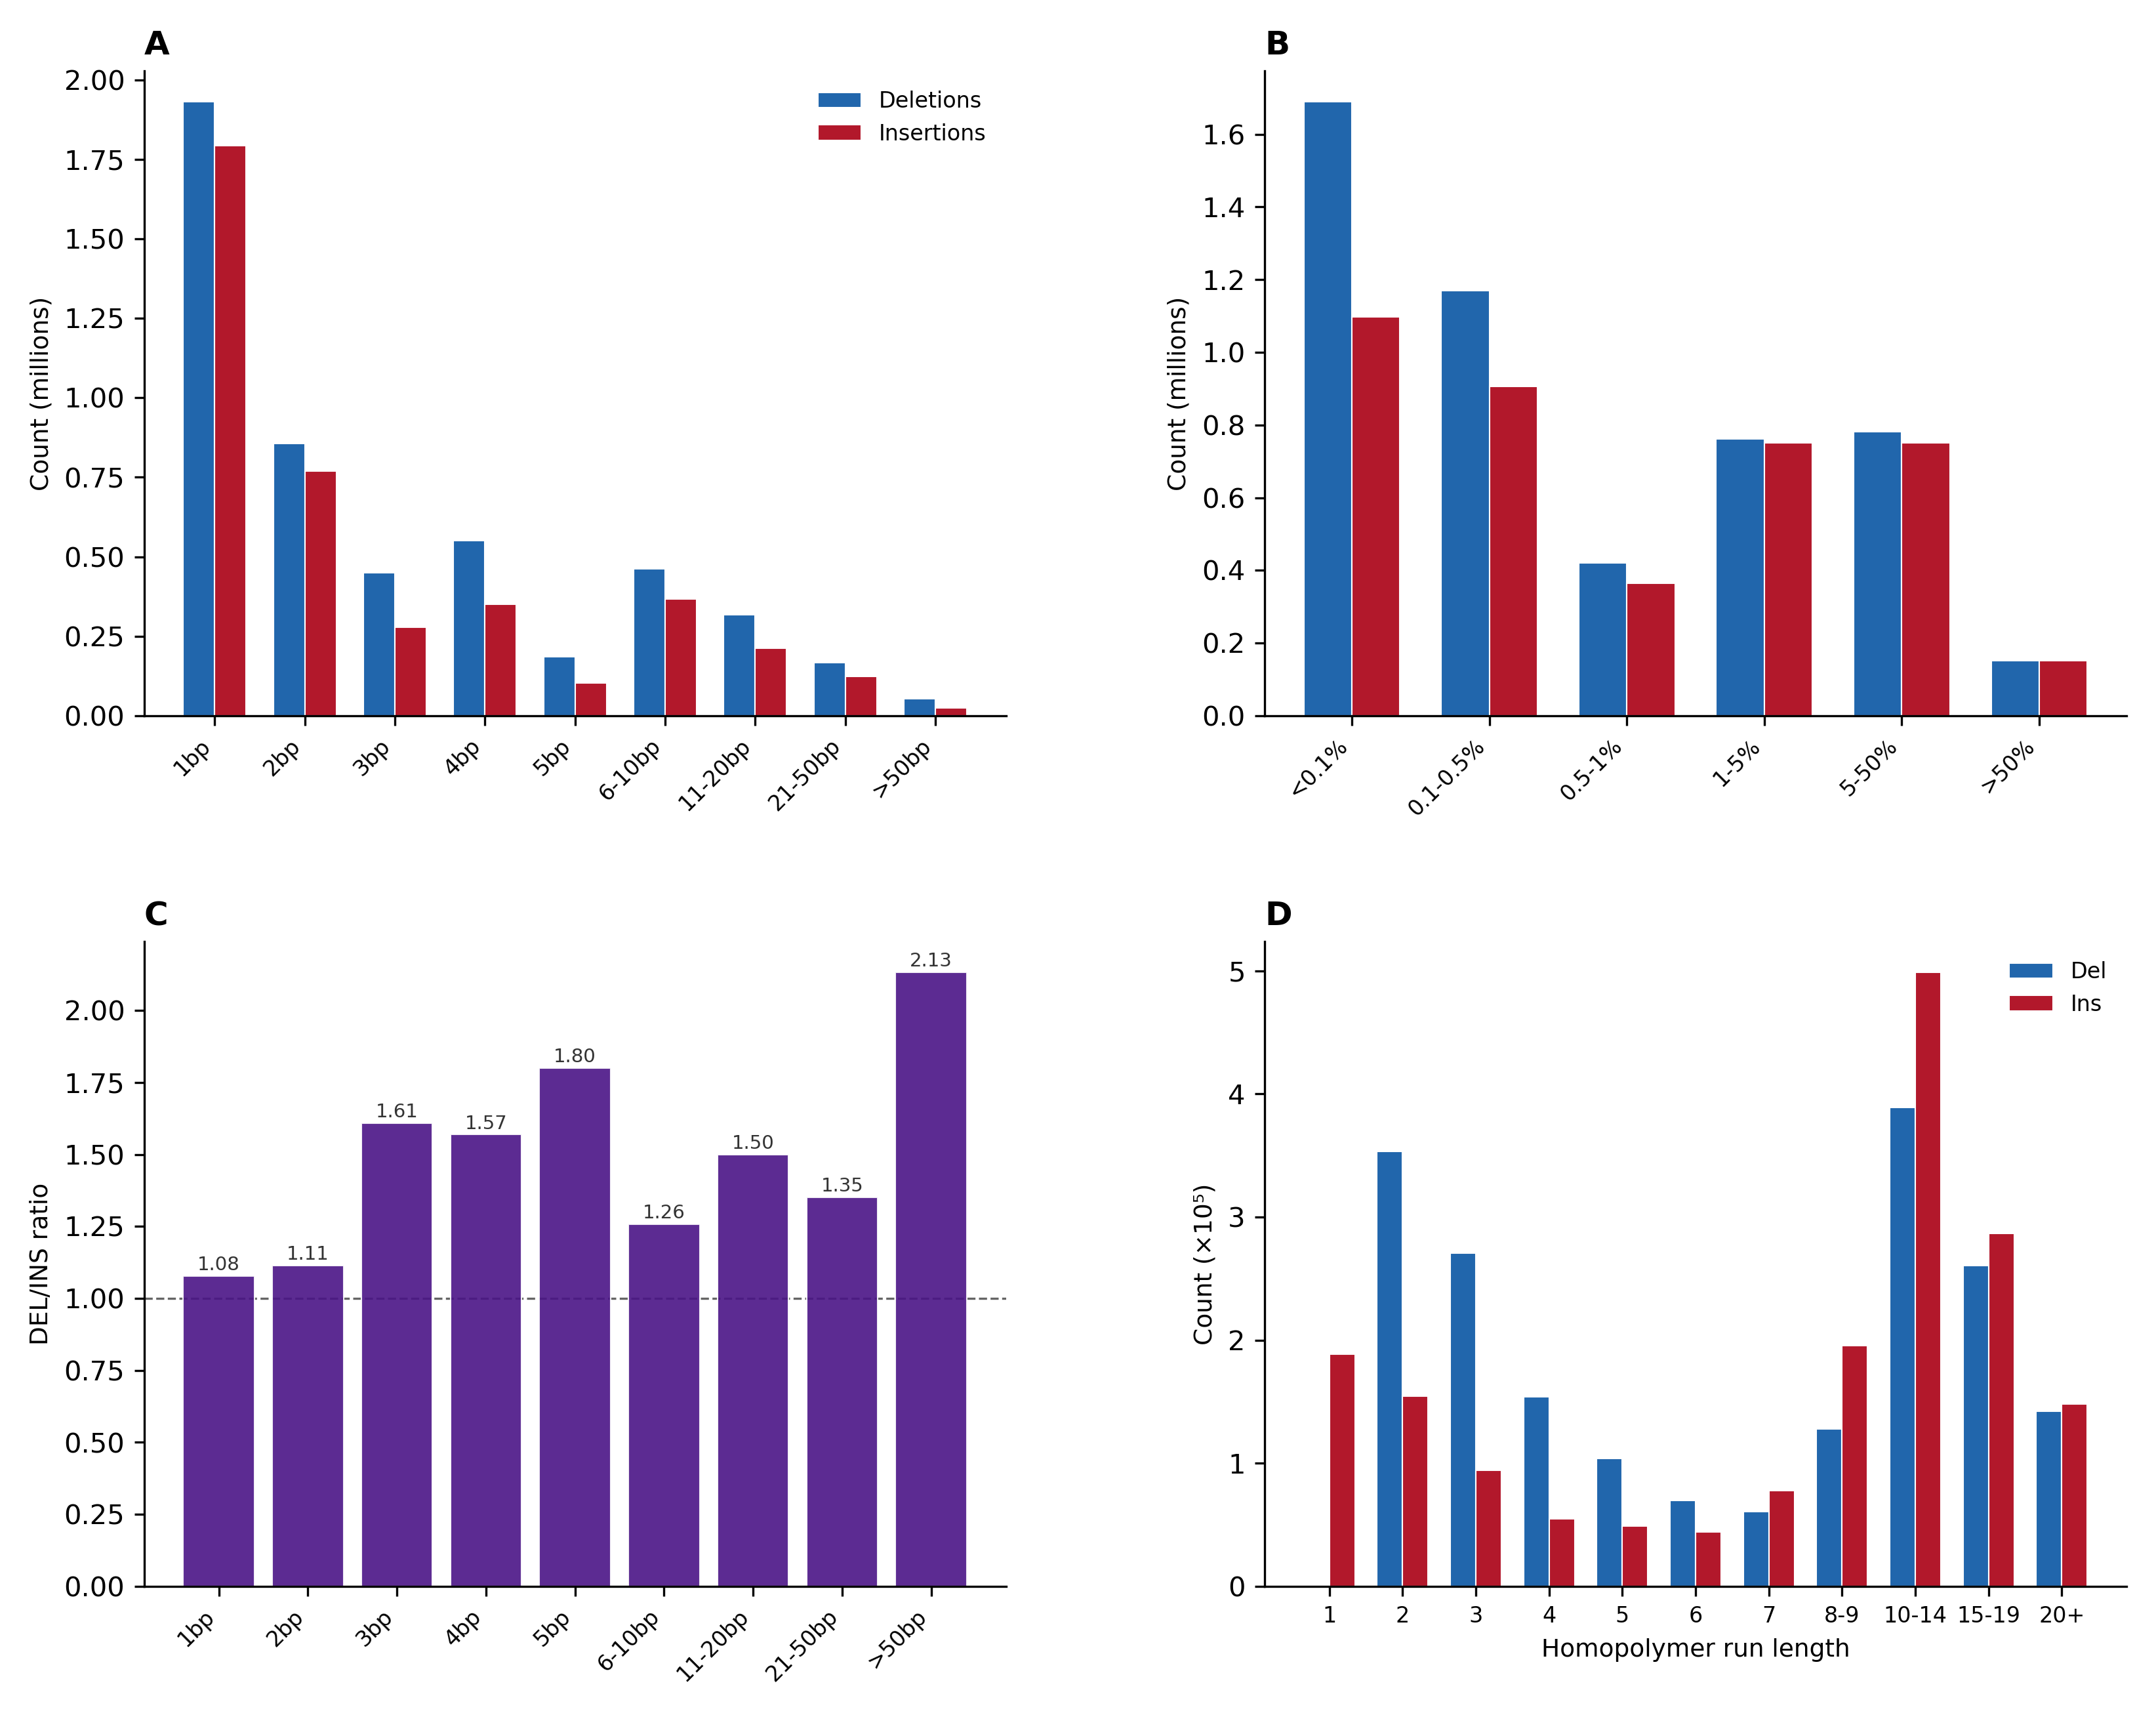
\includegraphics[width=\textwidth]{fig1_global_landscape.png}
\caption{\textbf{Genome-wide germline indel landscape.}
(\textbf{A})~Size distribution of deletions and insertions across 22 autosomes.
(\textbf{B})~Allele frequency spectrum of deletions and insertions.
(\textbf{C})~Deletion-to-insertion (DEL/INS) ratio as a function of indel size, showing increasing deletion bias with size.
(\textbf{D})~Distribution of 1\,bp indels by homopolymer run length at the variant position.
}
\label{fig:landscape}
\end{figure}

We identified 8,995,003 autosomal indels across 3,202 individuals, comprising 4,973,094 deletions (55.3\%) and 4,021,909 insertions (44.7\%), yielding a genome-wide DEL/INS ratio of 1.237 (Figure 1a). Single-nucleotide indels constituted the most abundant class (3,724,381; 41.4\% of all indels), with a strong preponderance of AT-context events (1,489,077 AT insertions and 1,437,482 AT deletions vs. 303,364 GC insertions and 494,458 GC deletions). The DEL/INS ratio exhibited marked size dependence, increasing from 1.08 at 1 bp to 2.13 at $>$50 bp (Figure 1c), consistent with a greater deletion bias for larger indels as previously observed \citep{kvikstad2007strong}.

The allele frequency spectrum was dominated by rare variants, with 31.0\% of indels having an allele frequency $< 0.1\%$ (singleton-like) and 23.1\% between 0.1--0.5\% (Figure 1b). Larger indels were enriched for rare allele frequencies compared to 1 bp indels, consistent with stronger purifying selection against larger indels.

Analysis of homopolymer context for 1 bp indels revealed that 94.9\% occurred within homopolymer runs (run length $\geq 2$), with 61.8\% in long homopolymers (run length $\geq 6$; Figure 1d). This pattern was more pronounced for AT-base indels than GC-base indels, reflecting the greater propensity for polymerase slippage at A/T homopolymers \citep{pearson2005repeat}. Insertions in long homopolymers outnumbered deletions (1,177,807 vs. 979,167 for hp $\geq 6$ in AT context), while deletions were relatively more common in shorter homopolymers.

\subsection{Population-Specific Indel Spectra}

\begin{figure}[!ht]
\centering
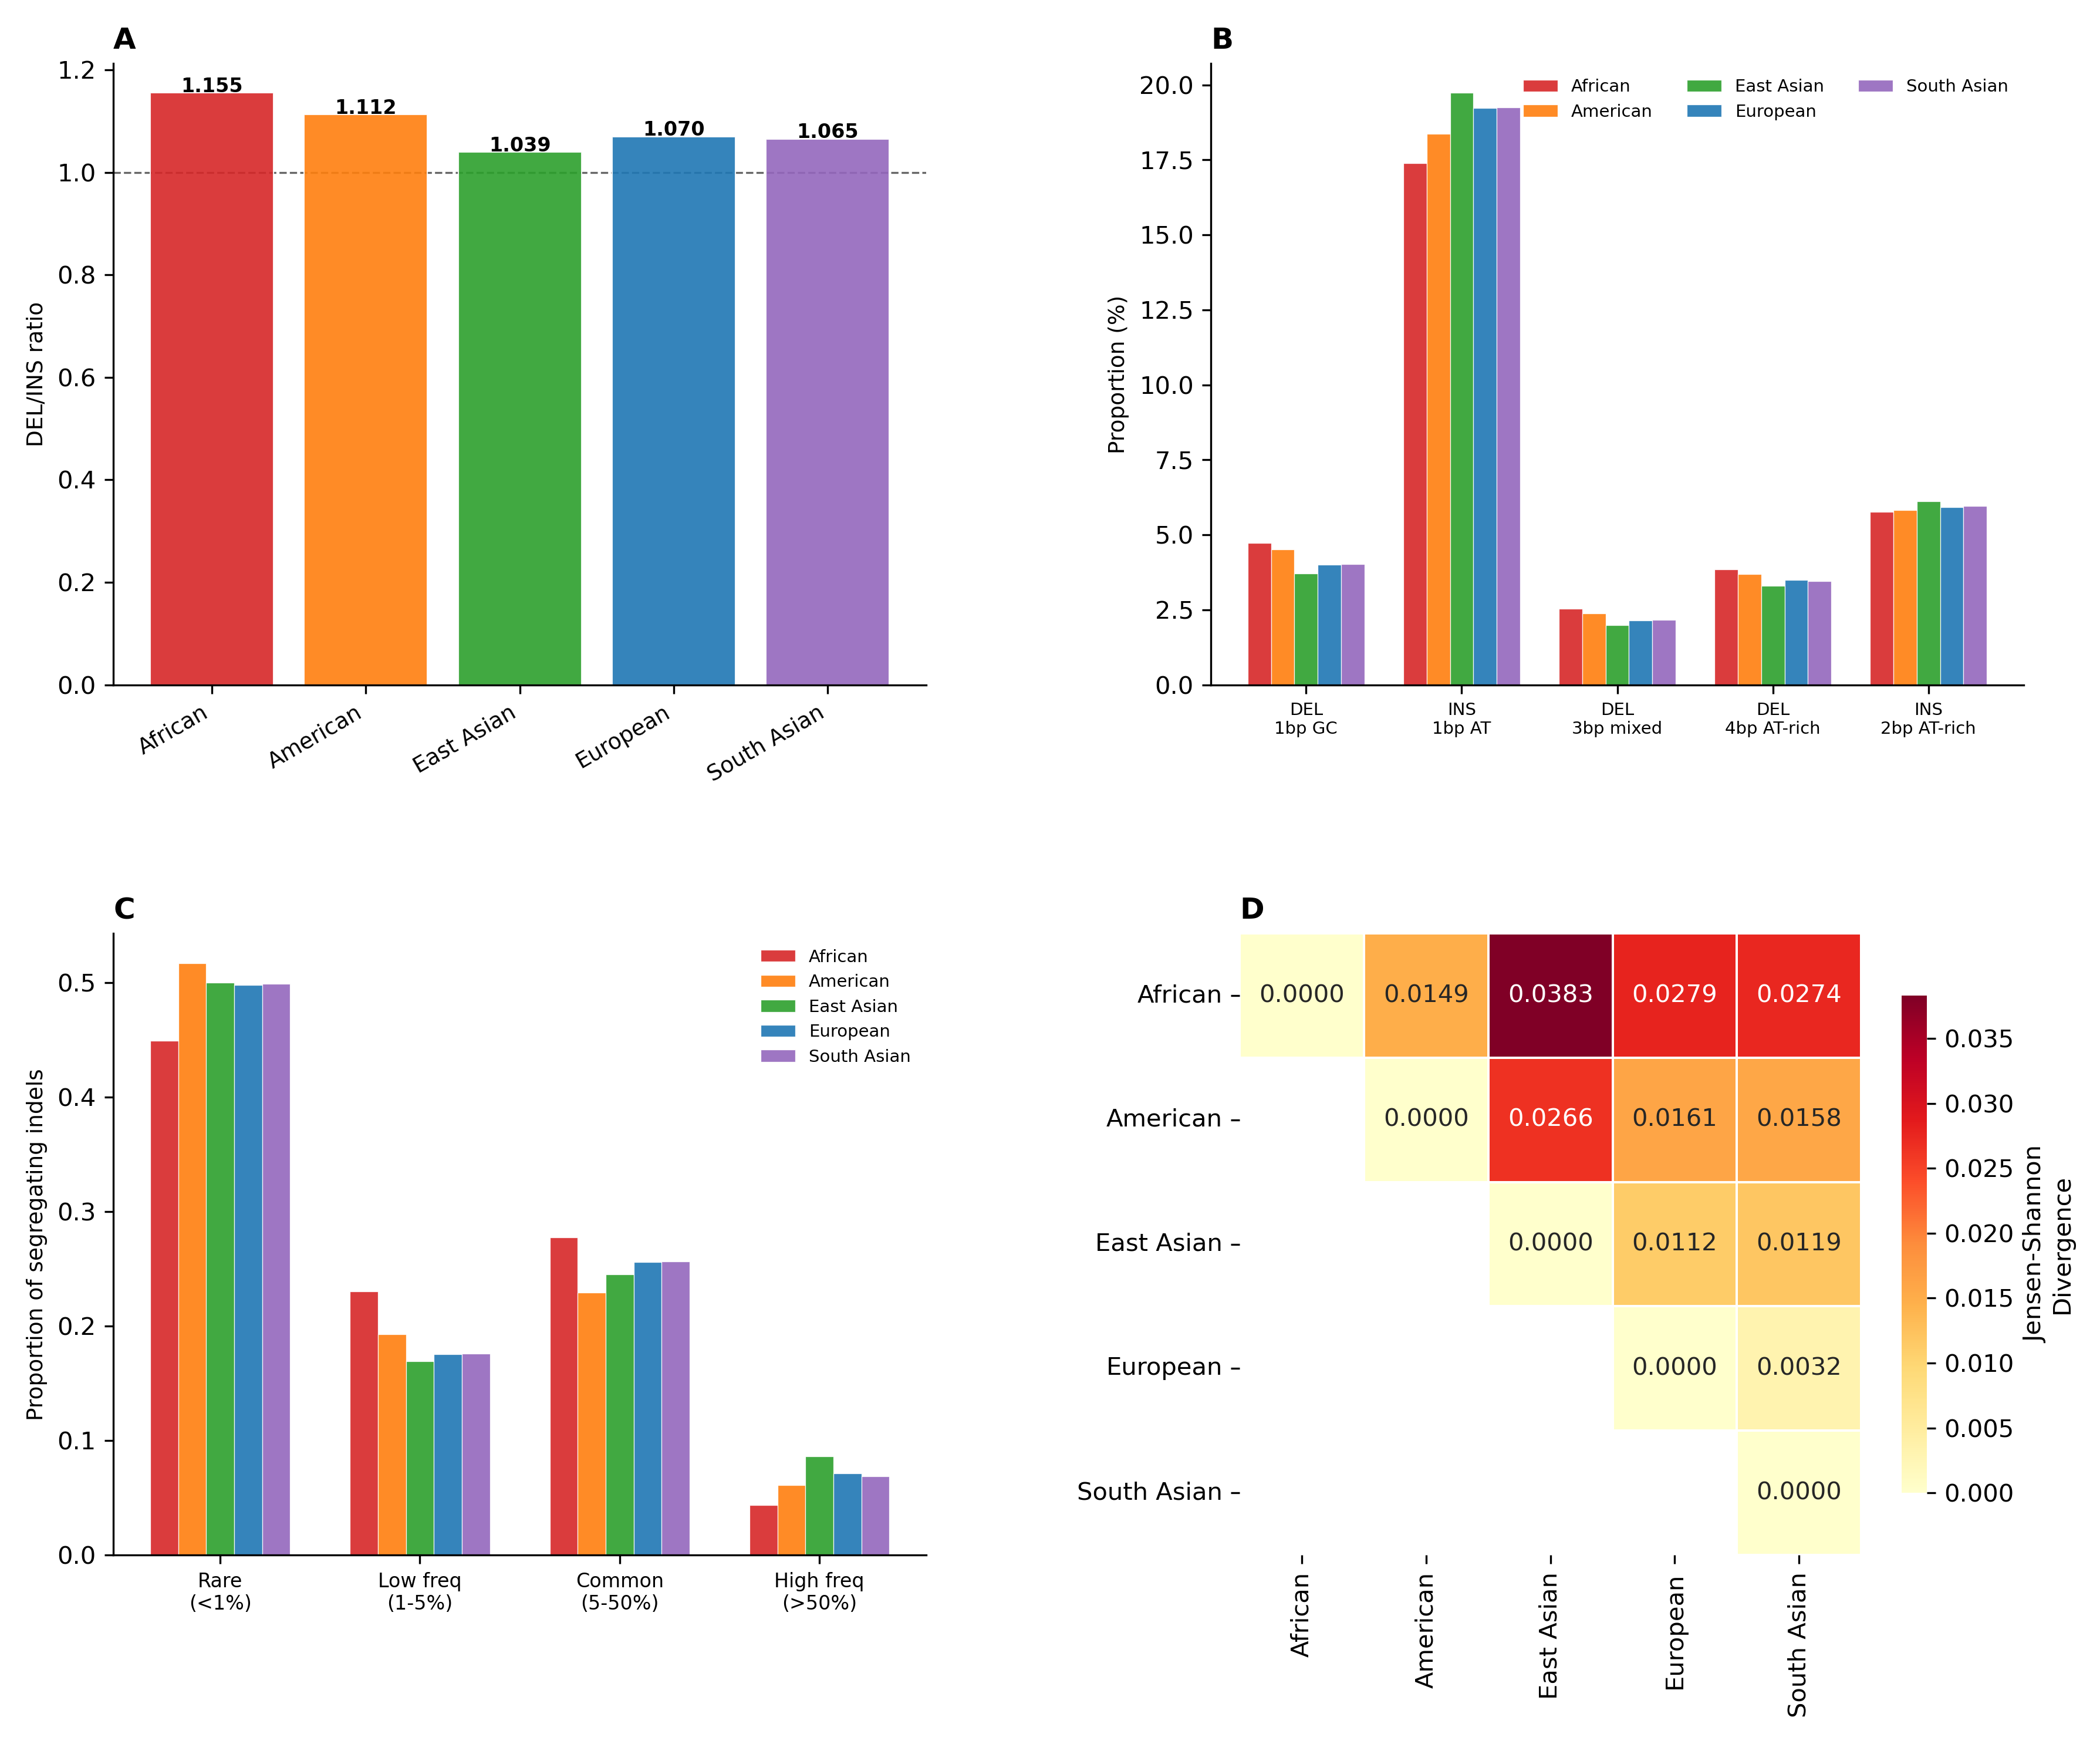
\includegraphics[width=\textwidth]{fig2_population_comparison.png}
\caption{\textbf{Population-specific indel spectrum comparison.}
(\textbf{A})~DEL/INS ratio across five continental super-populations.
(\textbf{B})~Proportions of key differentiated indel channels by super-population.
(\textbf{C})~Site frequency spectrum of segregating indels per super-population.
(\textbf{D})~Jensen-Shannon divergence between super-population indel spectra.
}
\label{fig:popcomp}
\end{figure}

We observed highly significant variation in indel spectra across the five continental super-populations ($\chi^2 = 3{,}465.58$, $df = 204$, $p < 10^{-300}$; Cram\'er's V = 0.020). All 52 channels showed significant differentiation after Bonferroni correction ($p_{\text{adj}} < 0.05$; Table 1), indicating pervasive population structure in the germline indel mutation spectrum.

\subsubsection{Deletion-to-Insertion Ratio Variation}

The DEL/INS ratio showed substantial variation across super-populations (Figure 2A): AFR exhibited the highest ratio (1.155), followed by AMR (1.113), EUR (1.070), SAS (1.065), and EAS (1.039). All ratios deviated significantly from unity (binomial test, all $p < 10^{-12}$). The 1.11-fold difference between AFR and EAS is striking and suggests differential contributions of deletion-generating vs. insertion-generating mutagenic processes across populations.

\subsubsection{Channel-Level Differentiation}

The most strongly differentiated channels involved 1 bp indels (Table 1; Figure 2a). Three key patterns emerged:

\begin{enumerate}
\item \textbf{GC-context deletion enrichment in African populations}: DEL\_1bp\_GC showed the highest FST-like differentiation, with AFR at 4.73\% vs. EAS at 3.72\% (1.27-fold enrichment). This extends to INS\_1bp\_GC (AFR: 3.26\% vs. EAS: 3.03\%, 1.08-fold). The excess of GC-context single-nucleotide deletions in AFR suggests elevated rates of mutagenic processes targeting GC-rich sequence contexts.

\item \textbf{AT-context insertion enrichment in East Asian populations}: INS\_1bp\_AT was the most strongly differentiated channel by absolute proportion, with EAS at 19.73\% vs. AFR at 17.39\% (1.13-fold). Given that the vast majority of 1 bp AT insertions occur in homopolymer runs, this pattern suggests population-specific variation in replication slippage rates at A/T homopolymers.

\item \textbf{Multi-base deletion enrichment in African populations}: Larger deletion classes---DEL\_3bp\_mixed (AFR: 2.52\% vs. EAS: 2.00\%, 1.26-fold), DEL\_4bp\_AT-rich (AFR: 3.75\% vs. EAS: 3.24\%, 1.16-fold), and DEL\_5bp\_AT-rich (AFR: 1.33\% vs. EAS: 1.09\%, 1.22-fold)---were consistently enriched in AFR. These multi-base deletions are less likely to arise from simple replication slippage, suggesting contributions from distinct repair-associated mutagenic processes.
\end{enumerate}

\subsubsection{Population Divergence}

Jensen-Shannon divergence (JSD) analysis revealed AFR as the most divergent super-population across all pairwise comparisons (JSD: AFR-EAS = 0.038, AFR-EUR = 0.028, AFR-AMR = 0.015), while EUR and SAS showed the smallest divergence (JSD = 0.003; Figure 2D). This pattern mirrors known demographic history but through the novel lens of the indel mutation spectrum: the out-of-Africa bottleneck and subsequent population divergence have left detectable signatures in the composition---not just the quantity---of indel variation. Cosine similarity analysis confirmed this pattern, with all pairwise similarities $> 0.9967$ but with AFR-EAS as the most dissimilar pair (cosine similarity = 0.9967).

\subsection{NMF Decomposition of Germline Indel Signatures}

\begin{figure}[!ht]
\centering
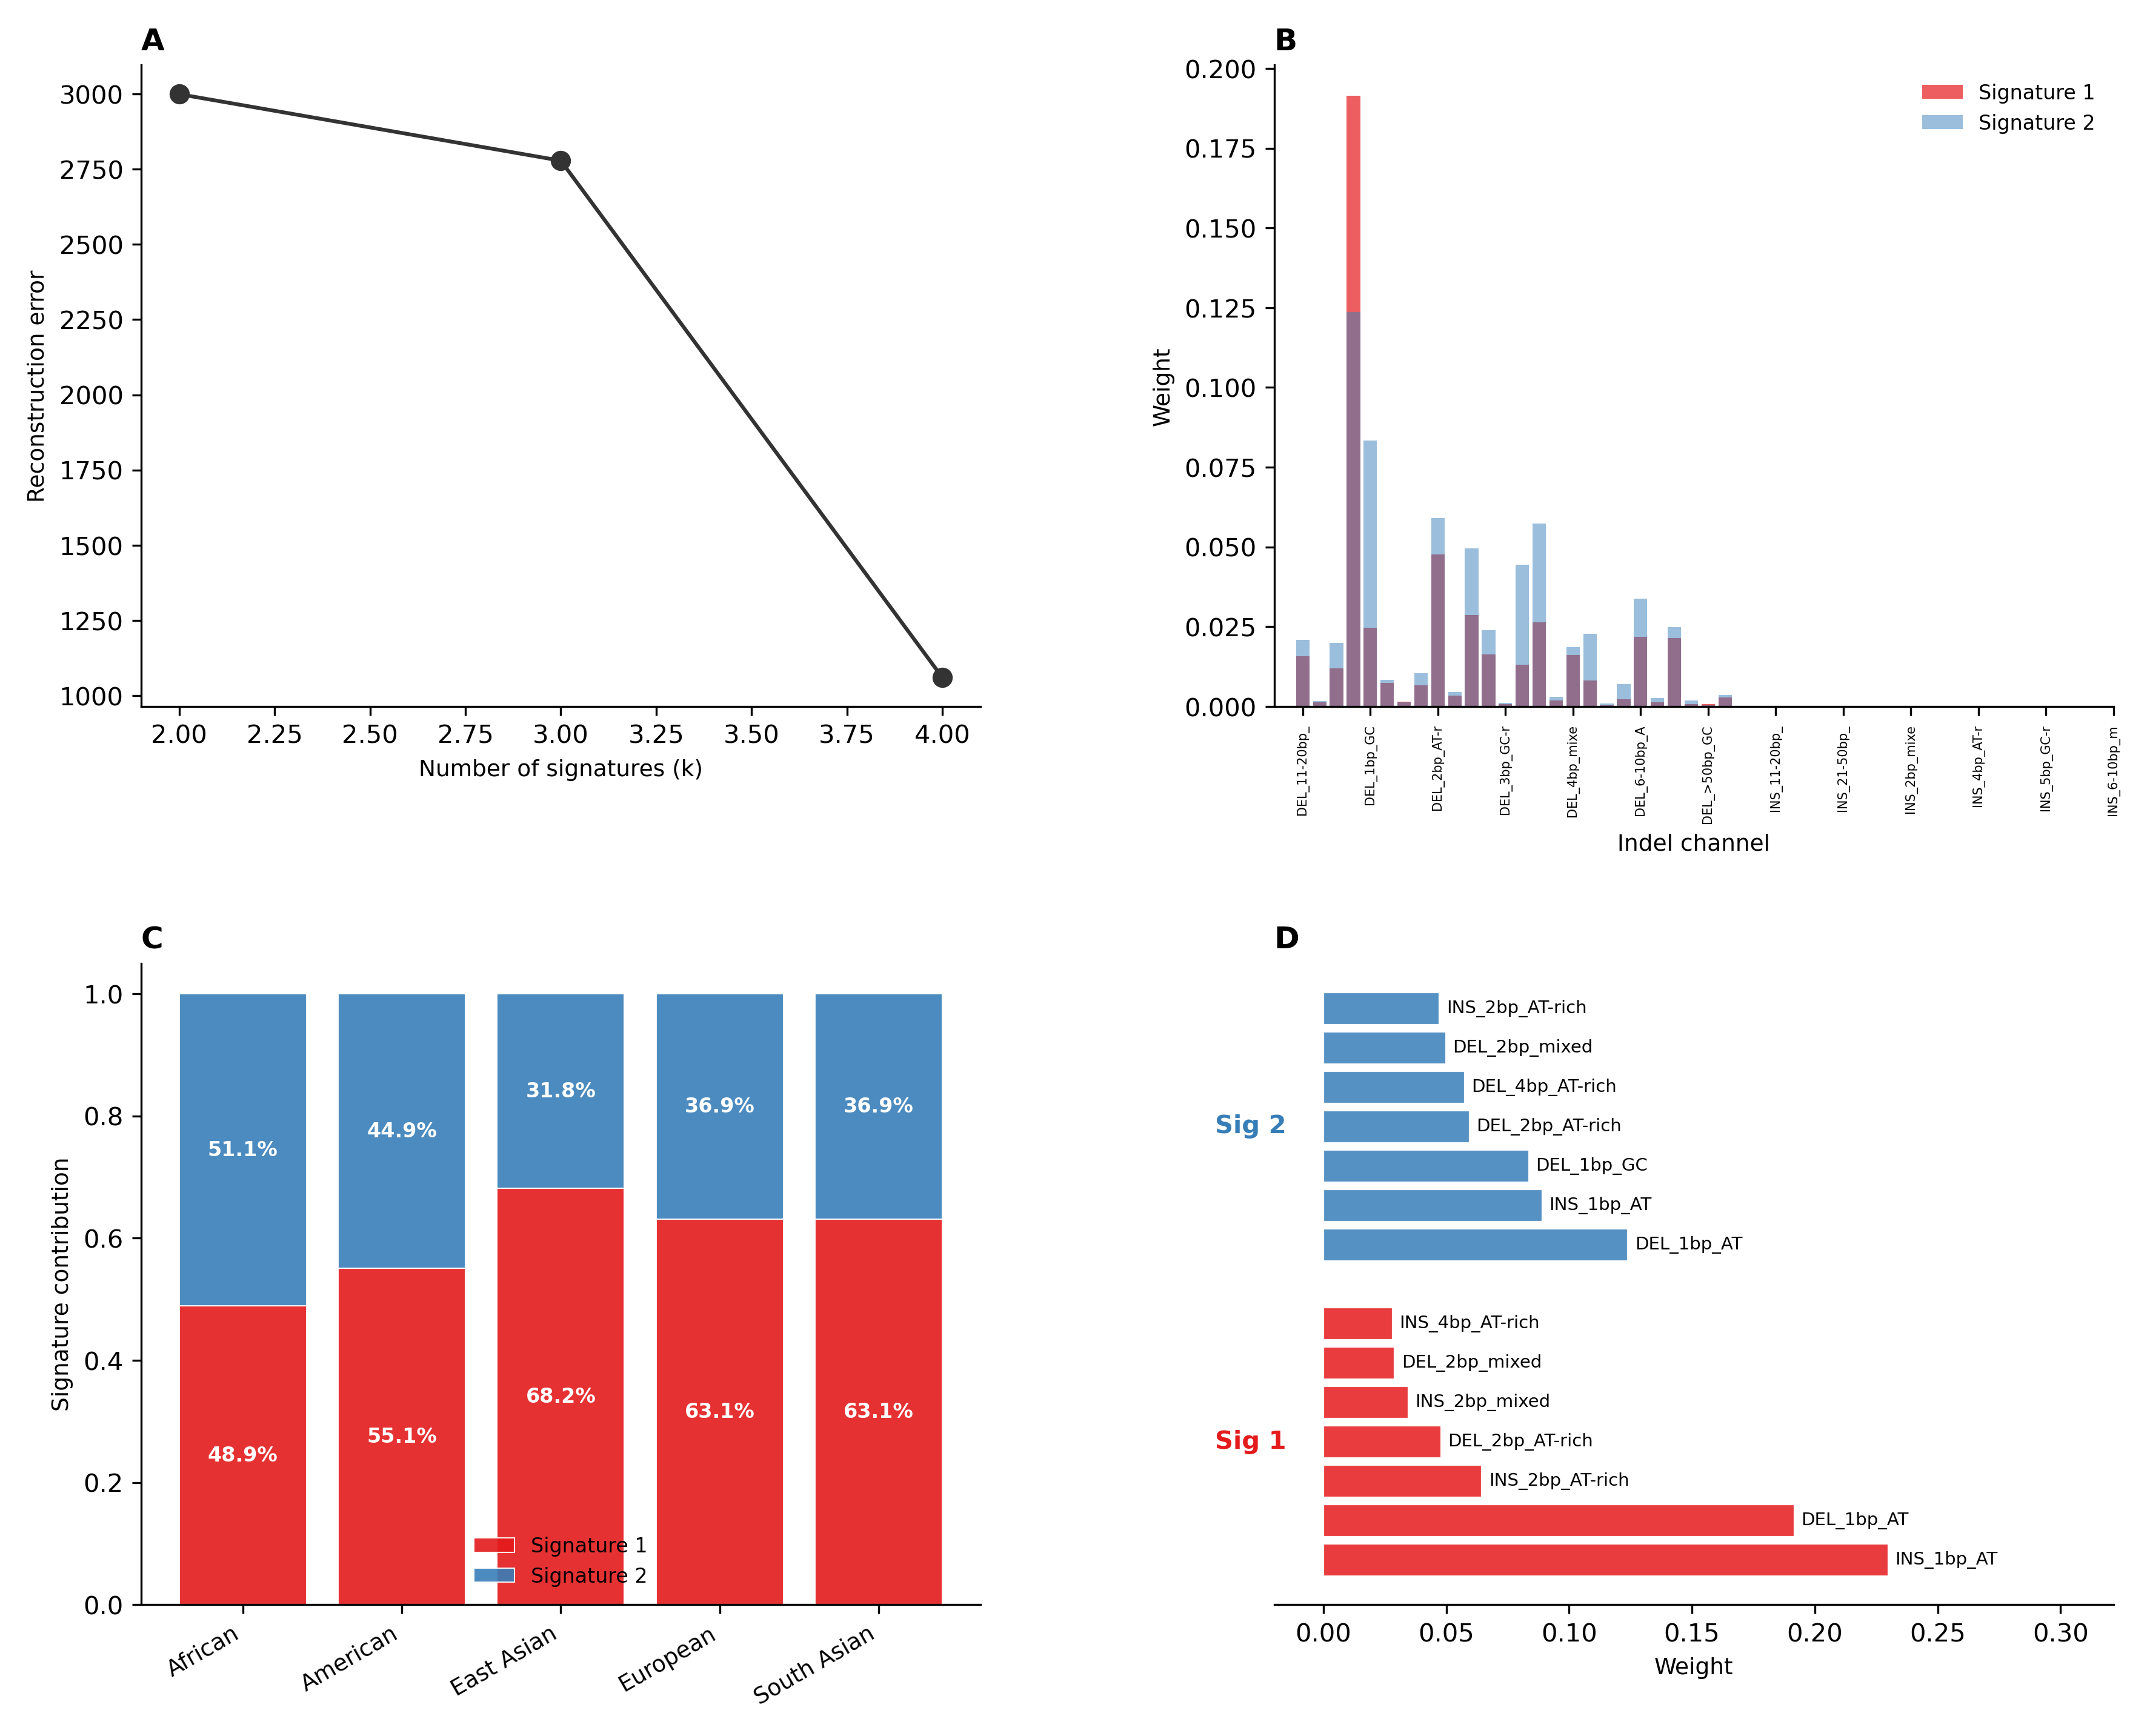
\includegraphics[width=\textwidth]{fig3_nmf_signatures.png}
\caption{\textbf{NMF decomposition of germline indel signatures.}
(\textbf{A})~Reconstruction error for NMF models with $k = 2$--4 signatures.
(\textbf{B})~Channel-level weight profiles for the two extracted signatures.
(\textbf{C})~Relative contribution of each signature across super-populations; percentages indicate the proportion of the indel spectrum explained by each signature.
(\textbf{D})~Top seven channels by weight for each signature.
}
\label{fig:nmf}
\end{figure}

To identify the component mutagenic processes contributing to population indel spectra, we applied NMF decomposition. A two-signature model ($k = 2$; reconstruction error = 1,610) provided the most interpretable decomposition (Figure 3):

\textbf{Signature 1 (AT-Slippage Signature)}: Dominated by INS\_1bp\_AT (weight = 0.231), DEL\_1bp\_AT (0.192), and INS\_2bp\_AT-rich (0.066). This signature captures the replication slippage process at AT-rich homopolymers, the predominant source of 1 bp germline indels. Its contribution was highest in EAS (68.2\%) and EUR (63.3\%), and lowest in AFR (48.9\%; Figure 3c).

\textbf{Signature 2 (GC-Deletion Signature)}: Enriched for DEL\_1bp\_GC (weight = 0.084), DEL\_1bp\_AT (0.123), and multi-base deletion channels. This signature captures non-homopolymer mutagenic processes including DNA repair errors and oxidative damage-associated deletions. Its contribution was highest in AFR (51.1\%) and AMR (44.7\%), and lowest in EAS (31.8\%).

The differential signature weights across populations provide a mechanistic framework for interpreting the observed spectral differences. The elevated Signature 2 contribution in AFR is consistent with either higher rates of GC-targeted mutagenesis (potentially related to environmental or lifestyle factors affecting DNA damage profiles) or differences in the efficiency of specific DNA repair pathways.

At $k = 4$, the model (reconstruction error = 527) further resolved the spectrum into four signatures, with an additional component capturing medium-sized (6--10 bp) indels with mixed base composition (Figure 3), but the two-signature model provided the clearest population separation.

\subsection{Allele Frequency Spectrum Variation}

The site frequency spectrum (SFS) of indels differed across super-populations (Figure 2c). AFR exhibited the largest proportion of rare indels ($< 1\%$ frequency; 44.7\% of segregating indels), consistent with larger effective population size. EAS showed the highest proportion of high-frequency indels ($> 50\%$: 8.7\%), reflecting the effects of genetic drift following the out-of-Africa bottleneck.

Population-private indels (segregating in only one super-population) were most abundant in AFR (223,604; 19.4\% of segregating indels), followed by EAS (9.7\%), SAS (9.1\%), EUR (4.4\%), and AMR (4.0\%). The high proportion of population-private indels in AFR reflects both greater total diversity and the deep coalescent history of African populations.

\subsection{Chromosomal Variation in Indel Density}

\begin{figure}[!ht]
\centering
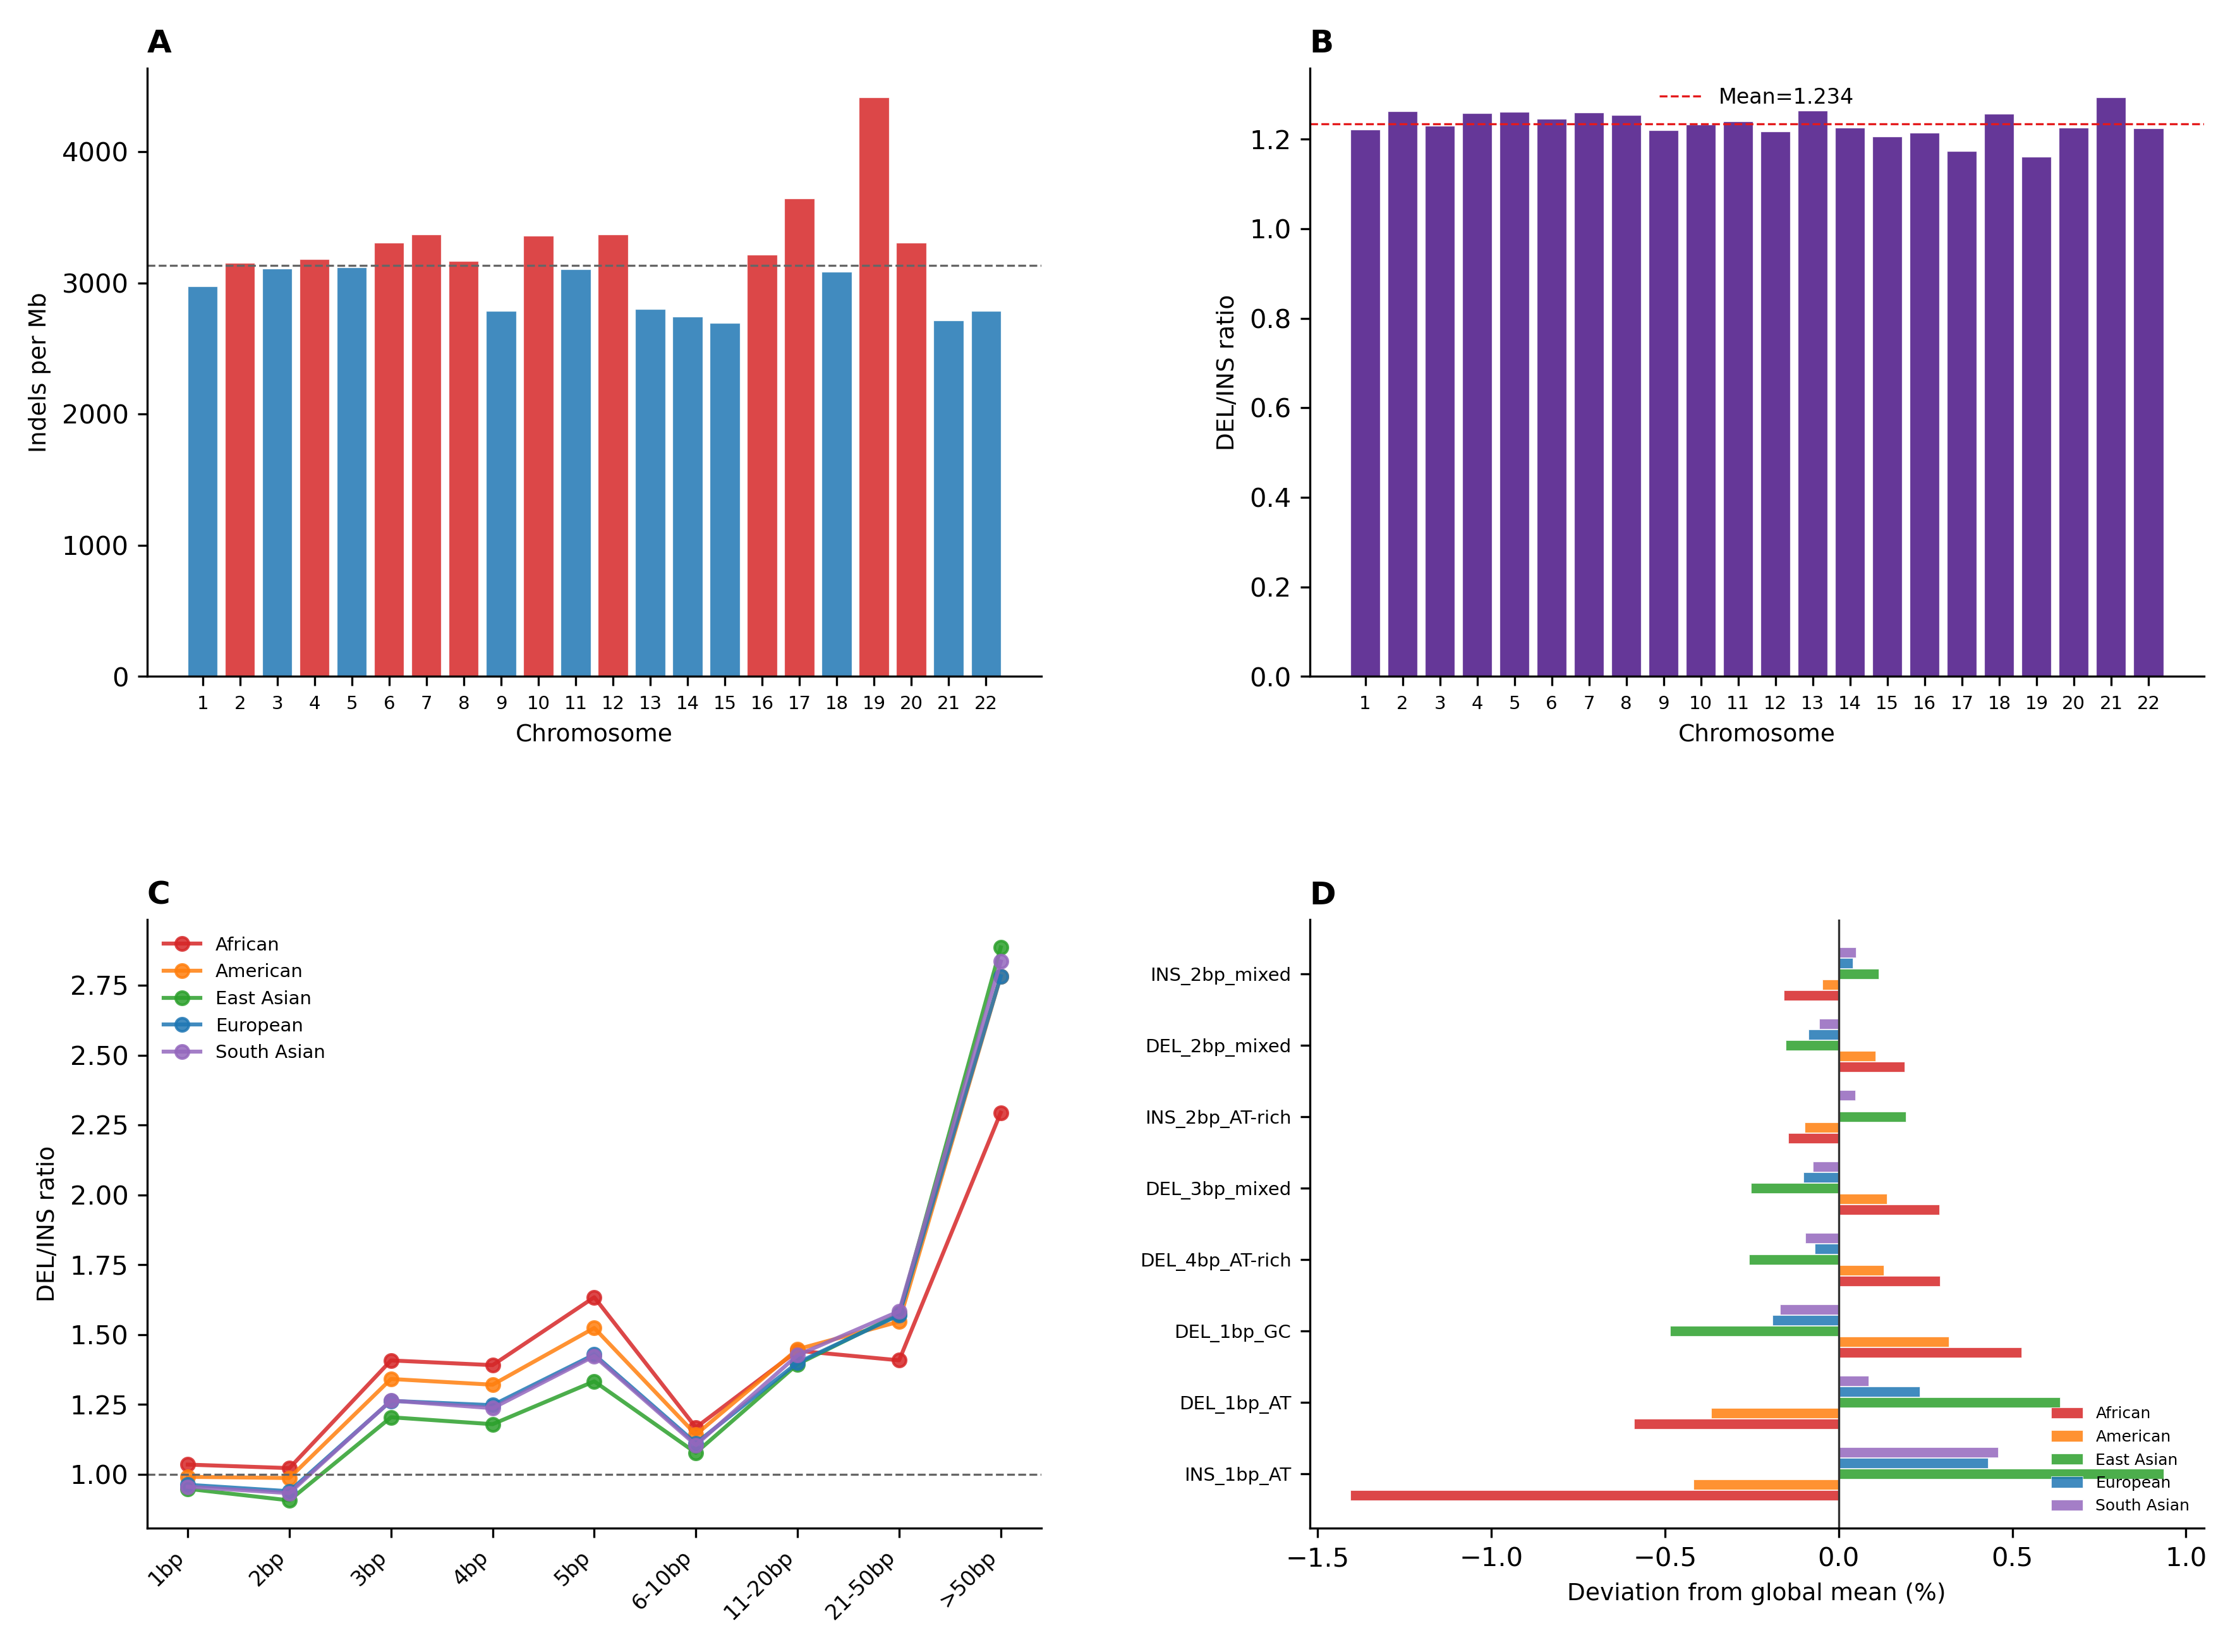
\includegraphics[width=\textwidth]{fig4_chromosomal_patterns.png}
\caption{\textbf{Chromosomal patterns of indel variation.}
(\textbf{A})~Indel density (indels per Mb) across 22 autosomes; dashed line indicates the median.
(\textbf{B})~DEL/INS ratio per chromosome; red dashed line shows the genome-wide mean.
(\textbf{C})~Size-dependent DEL/INS ratio stratified by super-population, showing consistent inter-population differences across all size classes.
(\textbf{D})~Deviation of each super-population's channel proportions from the global mean for the eight most variable channels.
}
\label{fig:chrom}
\end{figure}

Indel density varied across chromosomes from 2,716 per Mb (chr21) to 4,424 per Mb (chr19; Figure 4a). The DEL/INS ratio was relatively stable across chromosomes (range: 1.20--1.28; Figure 4b), suggesting that the genome-wide deletion bias is a general property rather than being driven by specific chromosomal regions. Chr19, known for its high gene density and GC content, exhibited among the highest indel densities, consistent with elevated mutagenesis in gene-dense regions.

\begin{figure}[!ht]
\centering
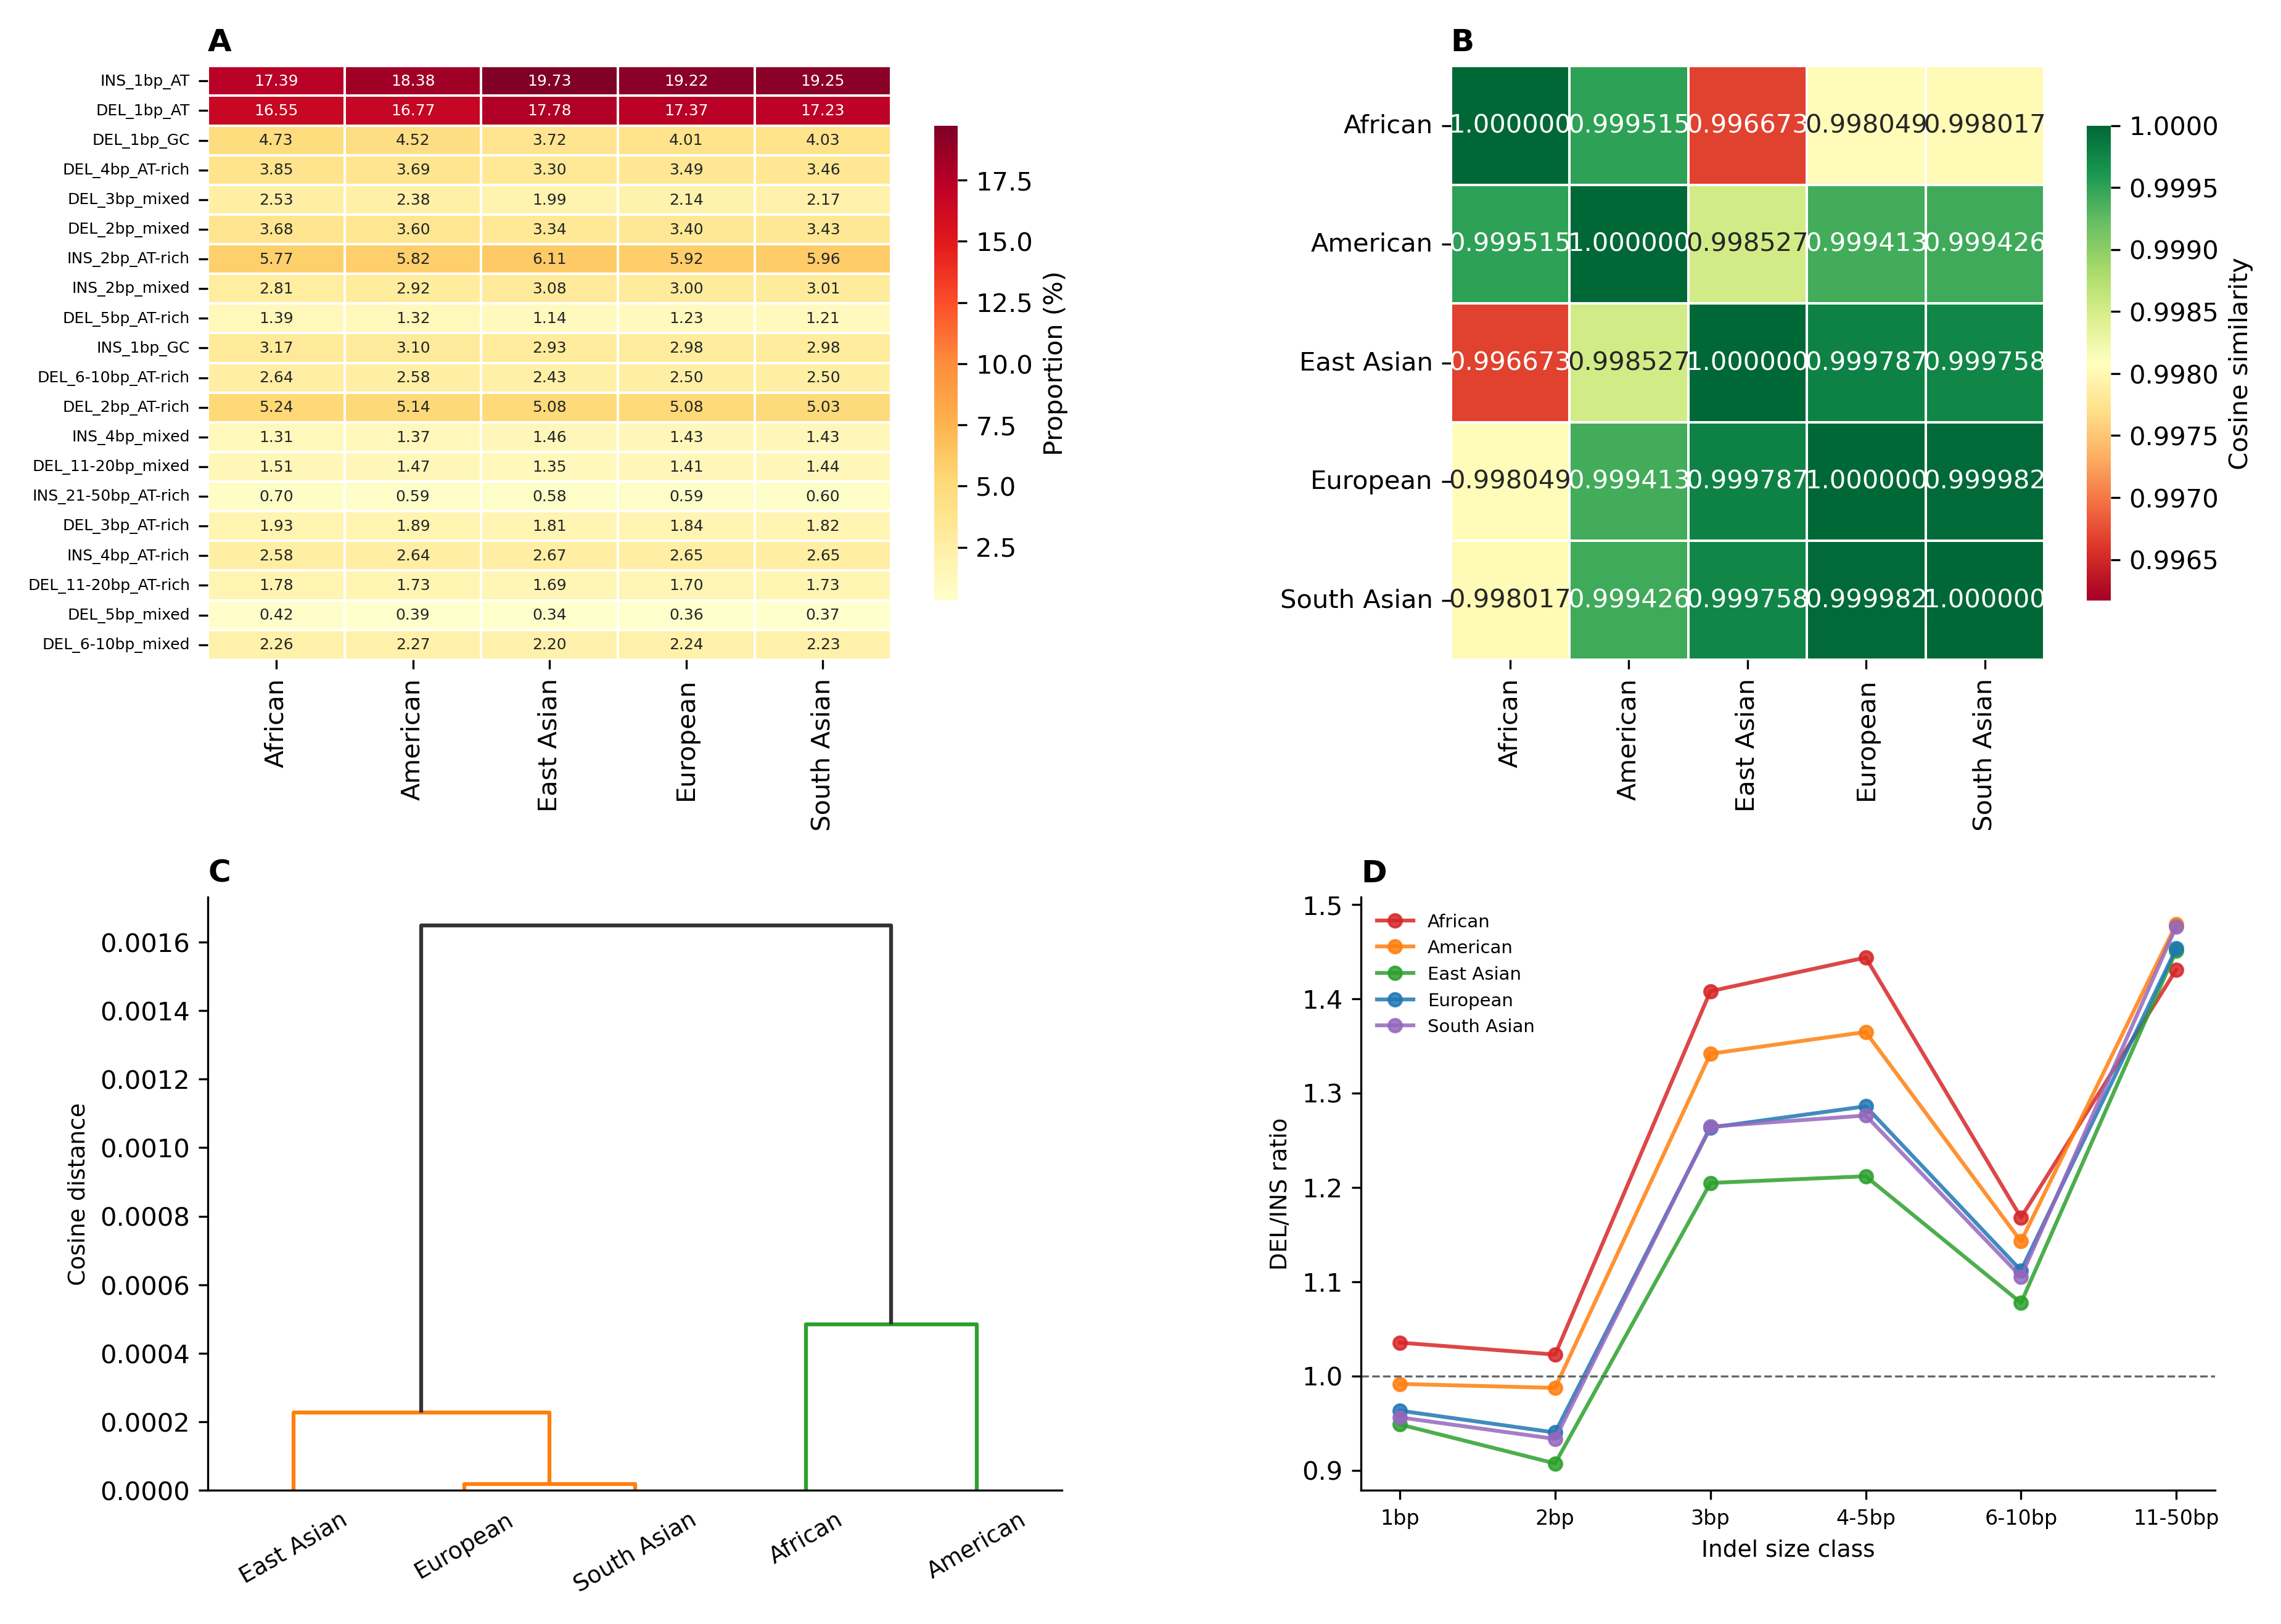
\includegraphics[width=\textwidth]{fig5_population_differentiation.png}
\caption{\textbf{Detailed population differentiation of indel spectra.}
(\textbf{A})~Heatmap of the 20 most variable indel channels across super-populations (proportions shown as percentages).
(\textbf{B})~Pairwise cosine similarity between super-population indel spectra.
(\textbf{C})~Hierarchical clustering (average linkage, cosine distance) of super-populations based on full indel spectra.
(\textbf{D})~DEL/INS ratio stratified by aggregated size class and super-population.
}
\label{fig:detail}
\end{figure}

\section{Discussion}

Our analysis reveals previously uncharacterized population-level variation in the germline indel mutation spectrum across diverse human populations. Using the high-coverage 1000 Genomes Project dataset, we demonstrate that the compositional spectrum of germline indels---defined by type, size, base composition, and sequence context---differs significantly across continental super-populations. These differences are not merely a consequence of varying total indel burden (which is expected from demographic history) but reflect population-specific variation in the relative contributions of distinct mutagenic processes.

\subsection{Differential Mutagenic Process Contributions}

The most striking finding is the elevated DEL/INS ratio and enrichment of GC-context deletions in African populations relative to other super-populations. Several non-mutually exclusive mechanisms could explain this pattern:

First, population-specific differences in oxidative DNA damage profiles could affect the rate of GC-targeted mutagenesis. 8-oxoguanine, a common oxidative lesion, preferentially affects guanine residues and can lead to deletions during error-prone repair \citep{david2007chemistry}. Environmental and lifestyle factors that influence oxidative stress levels could contribute to population-level variation in GC-deletion rates.

Second, differences in the efficiency or fidelity of specific DNA repair pathways---particularly mismatch repair (MMR) and base excision repair (BER)---could modulate the indel spectrum. Population-specific polymorphisms in DNA repair genes have been documented \citep{mathonnet2003variable} and could influence the relative rates of different indel-generating mechanisms.

Third, the enrichment of multi-base deletions (3--10 bp) in African populations suggests elevated rates of microhomology-mediated end joining (MMEJ) or alternative end joining pathways. These repair mechanisms generate deletions with characteristic microhomology signatures at junctions \citep{mcvey2008mmej} and may vary in activity across populations.

The relative enrichment of AT-context insertions in East Asian populations, predominantly occurring in homopolymer runs, points to population-specific variation in replication slippage rates or in the efficiency of post-replicative MMR at A/T homopolymers. This could reflect subtle population differences in DNA polymerase processivity or proofreading fidelity, potentially modulated by polymorphisms in polymerase subunits or accessory factors.

\subsection{Relationship to Known Population Structure}

The hierarchical clustering of populations based on indel spectra recapitulates the expected continental population structure (Figure 2d), with AFR as the most divergent group and EUR-SAS as the closest pair. This pattern is consistent with the out-of-Africa demographic model \citep{henn2012great} but provides complementary information to SNV-based population structure. Importantly, the spectral differences we observe are proportional rather than absolute---all populations share the same basic indel spectrum dominated by AT-context 1 bp events in homopolymers, but the relative proportions differ in ways that are statistically significant and biologically interpretable.

\subsection{Comparison with Somatic Indel Signatures}

The germline indel signatures identified by our NMF decomposition show notable parallels with COSMIC somatic indel signatures. Our Signature 1 (AT-slippage) shares features with COSMIC ID1 (insertion of T at long T homopolymers) and ID2 (deletion of T at long T homopolymers), both associated with replication slippage and defective MMR \citep{alexandrov2020repertoire}. Our Signature 2 (GC-deletion) has similarities with signatures associated with DNA damage-induced deletions. However, the germline context differs fundamentally from the somatic context: germline indels accumulate over generations and are subject to purifying selection, while somatic signatures reflect acute mutagenic processes within individual lifetimes. The population-level variation in germline signature contributions may reflect long-term differences in mutagenic exposures and repair capacities that have been shaped by evolutionary history.

\subsection{Limitations and Future Directions}

Several limitations should be noted. First, indel detection from short-read sequencing remains less accurate than SNV detection, particularly for larger indels and those in repetitive regions \citep{chaisson2019multi}. While the 30$\times$ coverage of the 1000GP dataset substantially improves indel calling compared to low-coverage data, some systematic biases may persist. Second, our NMF decomposition was performed on super-population-level spectra rather than individual-level spectra, limiting the resolution of signature extraction. Future work incorporating individual-level data with larger sample sizes could enable more refined signature decomposition. Third, our analysis focused on autosomes; extension to sex chromosomes and comparison with de novo mutation data could provide additional insights into the mechanisms of indel mutagenesis.

Future studies should integrate long-read sequencing data, which provides superior indel detection especially for larger structural variants, to validate and extend these findings. Additionally, examining the relationship between population-specific indel spectra and germline mutation rate variation, particularly in the context of de novo mutation studies, could help disentangle the contributions of mutation rate differences from selection and drift.

\section{Conclusion}

We present the first comprehensive population-stratified analysis of the germline indel mutation spectrum using high-coverage whole genome sequencing data from 3,202 globally diverse individuals. Our findings reveal significant population-specific variation in indel spectra, with African populations showing enrichment for GC-context deletions and multi-base deletions, and East Asian populations showing enrichment for AT-context insertions in homopolymer runs. NMF decomposition identifies two principal germline indel signatures with differential population contributions, suggesting population-specific variation in the rates of distinct mutagenic processes. These results extend our understanding of human mutational processes beyond SNVs and demonstrate that the indel mutation spectrum carries population-informative signals reflecting the interplay of mutagenesis, repair, and demographic history.

\section*{Data Availability}

The 1000 Genomes Project high-coverage dataset is publicly available from the International Genome Sample Resource (\url{https://www.internationalgenome.org/}). Analysis code is available upon request.

\section*{Acknowledgments}

This study used data generated by the 1000 Genomes Project and the International Genome Sample Resource. We thank the participants who contributed samples and the research teams who generated the sequencing and variant calling data.

\bibliographystyle{plainnat}

\begin{thebibliography}{99}

\bibitem[{1000 Genomes Project Consortium}(2015)]{1000genomes2015}
{1000 Genomes Project Consortium}. (2015). A global reference for human genetic variation. \textit{Nature}, 526(7571), 68--74.

\bibitem[Alexandrov et~al.(2013)]{alexandrov2013signatures}
Alexandrov, L.~B., Nik-Zainal, S., Wedge, D.~C., et~al. (2013). Signatures of mutational processes in human cancer. \textit{Nature}, 500(7463), 415--421.

\bibitem[Alexandrov et~al.(2020)]{alexandrov2020repertoire}
Alexandrov, L.~B., Kim, J., Haradhvala, N.~J., et~al. (2020). The repertoire of mutational signatures in human cancer. \textit{Nature}, 578(7793), 94--101.

\bibitem[Byrska-Bishop et~al.(2022)]{byrska2022high}
Byrska-Bishop, M., Evani, U.~S., Zhao, X., et~al. (2022). High-coverage whole-genome sequencing of the expanded 1000 Genomes Project cohort including 602 trios. \textit{Cell}, 185(18), 3426--3440.

\bibitem[Chaisson et~al.(2019)]{chaisson2019multi}
Chaisson, M.~J., Sanders, A.~D., Zhao, X., et~al. (2019). Multi-platform discovery of haplotype-resolved structural variation in human genomes. \textit{Nature Communications}, 10(1), 1784.

\bibitem[Chuzhanova et~al.(2003)]{chuzhanova2003meta}
Chuzhanova, N.~A., Anassis, E.~J., Ball, E.~V., Krawczak, M., \& Cooper, D.~N. (2003). Meta-analysis of indels causing human genetic disease: mechanisms of mutagenesis and the role of local DNA sequence complexity. \textit{Human Mutation}, 21(1), 28--44.

\bibitem[Danecek et~al.(2021)]{danecek2021twelve}
Danecek, P., Bonfield, J.~K., Liddle, J., et~al. (2021). Twelve years of SAMtools and BCFtools. \textit{GigaScience}, 10(2), giab008.

\bibitem[David et~al.(2007)]{david2007chemistry}
David, S.~S., O'Shea, V.~L., \& Kundu, S. (2007). Base-excision repair of oxidative DNA damage. \textit{Nature}, 447(7147), 941--950.

\bibitem[Henn et~al.(2012)]{henn2012great}
Henn, B.~M., Cavalli-Sforza, L.~L., \& Feldman, M.~W. (2012). The great human expansion. \textit{Proceedings of the National Academy of Sciences}, 109(44), 17758--17764.

\bibitem[Kvikstad et~al.(2007)]{kvikstad2007strong}
Kvikstad, E.~M., Tyekucheva, S., Chiaromonte, F., \& Makova, K.~D. (2007). A macaque's-eye view of human insertions and deletions: differences in mechanisms. \textit{PLoS Computational Biology}, 3(9), e176.

\bibitem[Lee \& Seung(1999)]{lee1999learning}
Lee, D.~D. \& Seung, H.~S. (1999). Learning the parts of objects by non-negative matrix factorization. \textit{Nature}, 401(6755), 788--791.

\bibitem[Levinson \& Gutman(1987)]{levinson1987slipped}
Levinson, G. \& Gutman, G.~A. (1987). Slipped-strand mispairing: a major mechanism for DNA sequence evolution. \textit{Molecular Biology and Evolution}, 4(3), 203--221.

\bibitem[Mathonnet et~al.(2003)]{mathonnet2003variable}
Mathonnet, G., Labuda, D., Meloche, C., Wambach, T., Krajinovic, M., \& Sinnett, D. (2003). Variable continental distribution of polymorphisms in the coding regions of DNA-repair genes. \textit{Journal of Human Genetics}, 48(12), 659--664.

\bibitem[McVey \& Lee(2008)]{mcvey2008mmej}
McVey, M. \& Lee, S.~E. (2008). MMEJ repair of double-strand breaks (director's cut): deleted sequences and alternative endings. \textit{Trends in Genetics}, 24(11), 529--538.

\bibitem[Mills et~al.(2011)]{mills2011natural}
Mills, R.~E., Pittard, W.~S., Mullaney, J.~M., et~al. (2011). Natural genetic variation caused by small insertions and deletions in the human genome. \textit{Genome Research}, 21(6), 830--839.

\bibitem[Montgomery et~al.(2013)]{montgomery2013mutation}
Montgomery, S.~B., Goode, D.~L., Kvikstad, E., et~al. (2013). The origin, evolution, and functional impact of short insertion-deletion variants identified in 179 human genomes. \textit{Genome Research}, 23(5), 749--761.

\bibitem[Mullaney et~al.(2010)]{mullaney2010small}
Mullaney, J.~M., Mills, R.~E., Pittard, W.~S., \& Bhattacharya, A. (2010). Small insertions and deletions (INDELs) in human genomes. \textit{Human Molecular Genetics}, 19(R2), R131--R136.

\bibitem[Pearson et~al.(2005)]{pearson2005repeat}
Pearson, C.~E., Nichol Edamura, K., \& Cleary, J.~D. (2005). Repeat instability: mechanisms of dynamic mutations. \textit{Nature Reviews Genetics}, 6(10), 729--742.

\bibitem[Pedregosa et~al.(2011)]{pedregosa2011scikit}
Pedregosa, F., Varoquaux, G., Gramfort, A., et~al. (2011). Scikit-learn: Machine learning in Python. \textit{Journal of Machine Learning Research}, 12, 2825--2830.

\bibitem[{pysam developers}(2024)]{pysam}
{pysam developers}. (2024). pysam: a Python module for reading, manipulating, and writing genomic data sets. \url{https://github.com/pysam-developers/pysam}.

\end{thebibliography}

\clearpage

\section*{Supplementary Tables}

\begin{table}[H]
\centering
\caption{Top 15 most population-differentiated indel channels. Chi-square statistics, Bonferroni-adjusted $p$-values, and proportions across super-populations are shown. All channels are significant at $\alpha = 0.05$ after correction.}
\label{tab:channels}
\small
\begin{tabular}{lrrrrrrrr}
\toprule
Channel & $\chi^2$ & $p_{\text{adj}}$ & AFR & AMR & EAS & EUR & SAS \\
\midrule
DEL\_1bp\_AT & 7187 & $<10^{-300}$ & 0.1654 & 0.1675 & 0.1776 & 0.1739 & 0.1724 \\
DEL\_1bp\_GC & 5985 & $<10^{-300}$ & 0.0482 & 0.0461 & 0.0380 & 0.0411 & 0.0413 \\
INS\_1bp\_AT & 5466 & $<10^{-300}$ & 0.1755 & 0.1858 & 0.1987 & 0.1945 & 0.1942 \\
DEL\_2bp\_AT-rich & 3583 & $<10^{-300}$ & 0.0518 & 0.0506 & 0.0501 & 0.0500 & 0.0496 \\
DEL\_4bp\_AT-rich & 3567 & $<10^{-300}$ & 0.0375 & 0.0362 & 0.0324 & 0.0344 & 0.0341 \\
DEL\_2bp\_mixed & 3134 & $<10^{-300}$ & 0.0364 & 0.0354 & 0.0329 & 0.0335 & 0.0338 \\
DEL\_3bp\_mixed & 3071 & $<10^{-300}$ & 0.0252 & 0.0235 & 0.0200 & 0.0214 & 0.0216 \\
INS\_2bp\_AT-rich & 2754 & $<10^{-300}$ & 0.0589 & 0.0596 & 0.0625 & 0.0607 & 0.0613 \\
INS\_1bp\_GC & 2561 & $<10^{-300}$ & 0.0326 & 0.0319 & 0.0303 & 0.0307 & 0.0308 \\
DEL\_6-10bp\_AT-rich & 2134 & $<10^{-300}$ & 0.0266 & 0.0261 & 0.0243 & 0.0251 & 0.0251 \\
DEL\_3bp\_AT-rich & 1495 & $<10^{-300}$ & 0.0191 & 0.0187 & 0.0178 & 0.0180 & 0.0179 \\
DEL\_5bp\_AT-rich & 1481 & $<10^{-300}$ & 0.0133 & 0.0128 & 0.0109 & 0.0117 & 0.0115 \\
DEL\_6-10bp\_mixed & 1437 & $<10^{-300}$ & 0.0246 & 0.0243 & 0.0240 & 0.0240 & 0.0240 \\
INS\_4bp\_AT-rich & 1298 & $<10^{-278}$ & 0.0253 & 0.0253 & 0.0264 & 0.0259 & 0.0259 \\
DEL\_11-20bp\_AT-rich & 1291 & $<10^{-276}$ & 0.0164 & 0.0162 & 0.0155 & 0.0155 & 0.0155 \\
\bottomrule
\end{tabular}
\end{table}

\begin{table}[H]
\centering
\caption{Summary of pairwise Jensen-Shannon divergence between super-population indel spectra.}
\label{tab:jsd}
\begin{tabular}{lrrrrr}
\toprule
 & AFR & AMR & EAS & EUR & SAS \\
\midrule
AFR & 0 & 0.0152 & 0.0378 & 0.0281 & 0.0273 \\
AMR & 0.0152 & 0 & 0.0262 & 0.0159 & 0.0156 \\
EAS & 0.0378 & 0.0262 & 0 & 0.0110 & 0.0117 \\
EUR & 0.0281 & 0.0159 & 0.0110 & 0 & 0.0034 \\
SAS & 0.0273 & 0.0156 & 0.0117 & 0.0034 & 0 \\
\bottomrule
\end{tabular}
\end{table}

\end{document}
